\documentclass[
  degree=bachelor,
  language=ru-en,
  bibstyle=gost-numeric
]{gostvkr-lua}

\usepackage{subcaption}
\usepackage{multirow}
\usepackage{makecell}
\usepackage{siunitx}
\usepackage{xcolor}
\usepackage{upquote}
\usepackage{listings}
\usepackage{algorithm}
\usepackage{algpseudocode}

\sisetup{
  output-decimal-marker={,},
  group-separator={\,},
  group-minimum-digits=4
}

\newcommand{\codeFontsDir}{fonts/fira-code/}
\newcommand{\requireCodeFont}[1]{%
  \IfFileExists{\codeFontsDir#1}{}{%
    \PackageError{main}{Не найден обязательный файл кодового шрифта: \codeFontsDir#1}{Скопируйте файлы Fira Code в локальную папку fonts/fira-code/.}%
  }%
}
\requireCodeFont{FiraCode-Regular.ttf}
\requireCodeFont{FiraCode-Medium.ttf}
\requireCodeFont{FiraCode-Bold.ttf}
\requireCodeFont{FiraCode-Retina.ttf}

\newfontfamily\codeFont[
  Path=\codeFontsDir,
  Extension=.ttf,
  UprightFont=FiraCode-Regular,
  BoldFont=FiraCode-Bold,
  ItalicFont=FiraCode-Retina,
  BoldItalicFont=FiraCode-Bold,
  Scale=0.92,
  RawFeature={-calt}
]{FiraCode-Regular}

\definecolor{lstBg}{HTML}{F8FAFD}
\definecolor{lstFrame}{HTML}{CFD7E3}
\definecolor{lstKeyword}{HTML}{0B4F9C}
\definecolor{lstComment}{HTML}{5C6B7A}
\definecolor{lstString}{HTML}{8A3B12}
\definecolor{lstNumber}{HTML}{7A8794}

\lstset{
  language=Python,
  basicstyle=\small\codeFont\color{black},
  keywordstyle=\bfseries\color{lstKeyword},
  commentstyle=\itshape\color{lstComment},
  stringstyle=\color{lstString},
  showstringspaces=false,
  numbers=left,
  numberstyle=\scriptsize\codeFont\color{lstNumber},
  numbersep=8pt,
  frame=single,
  framerule=0.4pt,
  rulecolor=\color{lstFrame},
  backgroundcolor=\color{lstBg},
  xleftmargin=6pt,
  xrightmargin=6pt,
  keepspaces=true,
  columns=fullflexible,
  breaklines=true,
  breakatwhitespace=false,
  upquote=true
}
\renewcommand{\lstlistingname}{Листинг}
\renewcommand{\lstlistlistingname}{Список листингов}
\floatname{algorithm}{Алгоритм}
\renewcommand{\listalgorithmname}{Список алгоритмов}

\gostsetup{
  direction = {09.03.01 Информатика и вычислительная техника},
  profile = {Технологии разработки программного обеспечения},
  fullname = {Фамилии Имени Отчества},
  course = {4},
  studyform = {очной},
  theme = {Здесь надо написать тему ВКР (смотрите правильные формулировки в приказах)},
  supervisor = {Учёная степень, учёное звание, должность руководителя ВКР\\Фамилия Имя Отчество},
  city = {Санкт-Петербург}
}


\addbibresource{references.bib}

\begin{document}

\maketitlepage

\tableofcontents

\makeintroduction
В современных условиях ускоренного роста цифровых сервисов обеспечение
их надёжности и производительности становится одной из ключевых задач разработки
программного обеспечения.
Нагрузочное тестирование позволяет выявить узкие места системы до её выхода
в промышленную эксплуатацию, оценить поведение сервиса при пиковых нагрузках
и проверить соответствие нефункциональным требованиям.
Среди широко применяемых инструментов --- Apache JMeter, Gatling, k6, Vegeta, hey.
Однако большинство из них требуют тяжёлых зависимостей,
ориентированы исключительно на HTTP или лишены встроенного веб-интерфейса
для визуального мониторинга теста в реальном времени.

\textbf{Актуальность} работы обусловлена потребностью в лёгком инструменте
нагрузочного тестирования, распространяемом в виде единого скомпилированного
бинарного файла, способном работать с HTTP и gRPC сервисами,
интегрироваться в конвейеры CI/CD через REST~API
и предоставлять наглядный веб-интерфейс для контроля хода тестирования.

\textbf{Объект исследования} --- процесс нагрузочного тестирования веб-сервисов
и gRPC-интерфейсов.

\textbf{Предмет исследования} --- программные методы разработки CLI
и веб-интерфейса инструмента нагрузочного тестирования с поддержкой HTTP и gRPC.

\textbf{Теоретическая значимость} работы заключается в систематизации подходов
к проектированию высокопроизводительных CLI-инструментов на языке Go,
анализе механизмов управления параллельными запросами
и ограничение скорости, а также в обосновании архитектурных решений
для потоковой передачи метрик через WebSocket.

\textbf{Практическая значимость} работы состоит в разработке готового к применению
инструмента Tsunami, который позволяет:
нагружать HTTP и gRPC сервисы с настраиваемой частотой запросов;
отслеживать метрики
в режиме реального времени через браузерный интерфейс;
экспортировать результаты в формате JSON для последующего анализа;
интегрировать тестирование в автоматизированные конвейеры через REST~API.
Разработанный инструмент распространяется в виде открытого программного
обеспечения для шести платформ через GitHub Releases и Homebrew,
что обеспечивает его доступность для широкого круга специалистов:
инженеров по качеству, DevOps-специалистов и преподавателей
дисциплин по тестированию программного обеспечения.
Кроме того, проект может служить учебным примером применения
Go-технологий (горутины, WebSocket, gRPC) при подготовке
специалистов в области разработки программного обеспечения.

\textbf{Цель} выпускной квалификационной работы --- разработать CLI-инструмент
и веб-интерфейс для системы нагрузочного тестирования HTTP и gRPC сервисов,
обеспечивающих гибкое управление нагрузкой и визуализацию метрик в реальном времени.

Для достижения поставленной цели необходимо решить следующие \textbf{задачи}:
\begin{enumerate}
  \item Провести сравнительный анализ существующих инструментов нагрузочного тестирования.
  \item Сформулировать функциональные и нефункциональные требования к разрабатываемому инструменту.
  \item Спроектировать архитектуру системы: движок нагрузочного тестирования, CLI-слой и серверную часть.
  \item Реализовать модуль нагрузочного тестирования с поддержкой протоколов HTTP и gRPC.
  \item Реализовать CLI-интерфейс для настройки, запуска и остановки нагрузочных тестов, а также вывода результатов тестирования в терминал.
  \item Разработать веб-интерфейс для запуска тестов и визуализации метрик в реальном времени.
  \item Провести тестирование разработанного инструмента и оценить его производительность.
\end{enumerate}

\textbf{Результатом} бакалаврской выпускной квалификационной работы является
инструмент нагрузочного тестирования Tsunami~--- программное средство
с интерфейсом командной строки и встроенным веб-приложением,
реализующее нагрузочное тестирование HTTP- и gRPC-сервисов
с отображением метрик в режиме реального времени.

\textbf{Структура бакалаврской выпускной квалификационной работы.}
Выпускная квалификационная работа состоит из введения, двух глав, заключения,
списка литературы и приложений.
В первой главе проводится анализ предметной области:
рассматриваются существующие инструменты нагрузочного тестирования,
обосновывается выбор технологий и проектируется архитектура системы.
Во второй главе описывается практическая реализация:
движок нагрузочного тестирования, CLI-интерфейс, серверная часть
с поддержкой WebSocket и веб-приложение на React.


\chapter{Аналитическая часть}
\section{Анализ существующих инструментов нагрузочного тестирования}

В условиях роста требований к надёжности веб-сервисов нагрузочное тестирование
стало неотъемлемой практикой в процессе разработки программного обеспечения.
Нагрузочное тестирование позволяет воспроизвести условия реальной эксплуатации,
выявить узкие места производительности и оценить поведение сервиса при пиковом
трафике ещё до развёртывания в промышленной среде~\cite{gost7322017}.
Без систематического проведения нагрузочных испытаний разработчики рискуют
обнаружить деградацию производительности уже в условиях промышленной эксплуатации,
когда стоимость устранения проблем многократно возрастает.

Существующие инструменты нагрузочного тестирования можно разделить на несколько
категорий: тяжёлые корпоративные решения с графическим интерфейсом,
скриптовые инструменты на базе JVM, лёгкие CLI-утилиты и облачные платформы.
Для обоснования разработки собственного инструмента был проведён сравнительный
анализ наиболее распространённых открытых решений.

\textbf{Apache JMeter}~--- один из старейших и наиболее функциональных инструментов
нагрузочного тестирования с открытым исходным кодом~\cite{jmeter}.
Распространяется в виде Java-приложения и требует наличия JVM версии~11 и выше.
JMeter поддерживает широкий спектр протоколов: HTTP, HTTPS, FTP, JDBC, LDAP и другие,
обладает развитым графическим интерфейсом для визуального конструирования
планов тестирования.
Вместе с тем инструмент отличается высокой сложностью настройки: конфигурация
хранится в XML-формате, а дистрибутив занимает более 60~МБ.
Потребление памяти JVM существенно ограничивает масштабируемость
на машинах с ограниченными ресурсами, а интеграция в конвейеры CI/CD требует
дополнительной настройки плагинов и сторонних инструментов разбора отчётов.

\textbf{Gatling}~--- высокопроизводительный инструмент нагрузочного тестирования,
ориентированный на HTTP-протокол~\cite{gatling}.
Написан на Scala и работает на платформе JVM, что влечёт те же зависимости
рантайма, что и Apache JMeter.
Сценарии тестирования описываются на предметно-ориентированном языке (DSL)
на основе Scala, что требует от пользователя базовых знаний этого языка.
Gatling генерирует подробные HTML-отчёты с перцентилями задержки и графиками
распределения, однако поддержка gRPC доступна только в коммерческой редакции
Gatling Enterprise.

\textbf{k6}~--- современный инструмент нагрузочного тестирования с открытым исходным
кодом, разработанный компанией Grafana Labs~\cite{k6}.
Бинарный файл написан на языке Go, однако сценарии нагрузочных тестов описываются
на JavaScript (TypeScript), что требует знания этого языка и усложняет автоматизацию
в простых сценариях.
k6 поддерживает HTTP, WebSocket и gRPC, предоставляет встроенную интеграцию с Grafana
Cloud для визуализации результатов.
Установка предполагает использование предкомпилированных бинарей или среды Node.js
при написании расширений.

\textbf{Vegeta}~--- минималистичный HTTP-инструмент нагрузочного тестирования,
написанный на языке Go~\cite{vegeta}.
Распространяется в виде единого бинарного файла без внешних зависимостей,
что делает его удобным для CI/CD-сред.
Vegeta поддерживает только протокол HTTP и не имеет встроенного веб-интерфейса
для мониторинга хода теста в реальном времени.
Конфигурация передаётся через стандартный ввод в текстовом формате,
что ограничивает сценарии использования динамически формируемыми нагрузками.

\textbf{hey}~--- простой HTTP-инструмент нагрузочного тестирования на Go,
ориентированный на быструю проверку производительности одного эндпоинта~\cite{hey}.
Не поддерживает gRPC, лишён веб-интерфейса и расширенных метрик ошибок;
результат выводится только в виде текстового отчёта по завершении теста,
что не позволяет отслеживать динамику метрик в ходе нагрузочного испытания.

Результаты сравнительного анализа представлены в таблице~\ref{tab:ch1-tools}.

\begin{table}[tbp]
  \centering
  \caption{Сравнительный анализ инструментов нагрузочного тестирования}
  \label{tab:ch1-tools}
  \small
  \begin{tabular}{@{}p{0.14\linewidth}p{0.13\linewidth}p{0.13\linewidth}p{0.12\linewidth}p{0.14\linewidth}p{0.18\linewidth}@{}}
    \toprule
    Инструмент     & Язык / рантайм & Протоколы      & Интерфейс & Зависимости       & Веб-интерфейс \\
    \midrule
    Apache JMeter  & Java (JVM)     & HTTP, gRPC, FTP & GUI, CLI  & JVM 11+           & Сторонние плагины \\
    Gatling        & Scala (JVM)    & HTTP            & CLI, HTML & JVM 11+           & HTML-отчёт (статика) \\
    k6             & Go + JS        & HTTP, WS, gRPC  & CLI       & Node.js (скрипты) & Grafana Cloud \\
    Vegeta         & Go             & HTTP            & CLI       & Нет               & Отсутствует \\
    hey            & Go             & HTTP            & CLI       & Нет               & Отсутствует \\
    \textbf{Tsunami} & \textbf{Go}  & \textbf{HTTP, gRPC} & \textbf{CLI + веб} & \textbf{Нет} & \textbf{Встроенный} \\
    \bottomrule
  \end{tabular}
\end{table}

Анализ таблицы~\ref{tab:ch1-tools} позволяет сделать следующие выводы.
Инструменты на базе JVM (JMeter, Gatling) обладают широким функционалом, однако
требуют наличия Java-рантайма и потребляют значительный объём оперативной памяти,
что затрудняет их использование в контейнерных и CI/CD-средах.
Инструменты на Go (Vegeta, hey) являются лёгкими и не имеют зависимостей,
однако ограничены только протоколом HTTP и не предоставляют визуального мониторинга.
k6 поддерживает gRPC и имеет интеграцию с Grafana, но для написания сценариев
требует знания JavaScript, а встроенная визуализация доступна только через
платный облачный сервис.

Таким образом, на рынке отсутствует инструмент, объединяющий лёгкость и
отсутствие зависимостей Go-бинаря, поддержку HTTP и gRPC в одном исполняемом файле
и встроенный веб-интерфейс с потоковой передачей метрик в реальном времени.
Данный пробел и определяет необходимость разработки инструмента Tsunami.


\section{Требования к разрабатываемому инструменту}

На основе проведённого анализа предметной области и выявленных недостатков
существующих решений были сформулированы требования к разрабатываемому
инструменту нагрузочного тестирования.

\textbf{Функциональные требования:}
\begin{enumerate}
  \item Поддержка нагрузочного тестирования HTTP-сервисов с настраиваемыми
    методом запроса, заголовками и телом.
  \item Поддержка нагрузочного тестирования gRPC-сервисов с возможностью
    указания .proto-файла или использования server reflection.
  \item Гибкое управление частотой запросов в формате \texttt{N/Vunit}
    (например, \texttt{100/1s}, \texttt{50/500ms}).
  \item Настройка числа параллельных воркеров и размера пула HTTP-соединений.
  \item Сбор и отображение метрик: общее число запросов, успехи, отказы,
    минимальная, средняя и максимальная задержка,
    перцентили p50, p95, p99, p99.9,
    пропускная способность (RPS), объём переданных данных.
  \item Классификация ошибок по типам: таймаут, отказ в соединении,
    ошибка DNS, ошибка TLS, прочие.
  \item Разбивка результатов по HTTP-кодам ответов.
  \item Веб-интерфейс для запуска тестов и визуализации метрик в реальном времени.
  \item REST~API для управления тестами из внешних систем (CI/CD).
  \item Экспорт результатов в формате JSON.
  \item Встроенная поддержка graceful shutdown по сигналам SIGINT/SIGTERM.
\end{enumerate}

\textbf{Нефункциональные требования:}
\begin{enumerate}
  \item Распространение в виде единого скомпилированного бинарного файла
    без внешних зависимостей рантайма.
  \item Кросс-платформенная поддержка: Linux, macOS, Windows;
    архитектуры amd64 и arm64.
  \item Корректная работа при целевой частоте не менее 1000~RPS
    при 50 параллельных воркерах на современном серверном оборудовании.
  \item Потокобезопасный сбор метрик без потери данных при высокой нагрузке.
  \item Задержка доставки метрик через WebSocket~--- не более 100~мс.
\end{enumerate}

Для наглядного представления вариантов использования системы была составлена
диаграмма прецедентов (рисунок~\ref{fig:ch1-usecase}), отражающая взаимодействие
двух категорий пользователей: CLI-пользователя и веб-пользователя.

\begin{figure}[tbp]
  \centering
  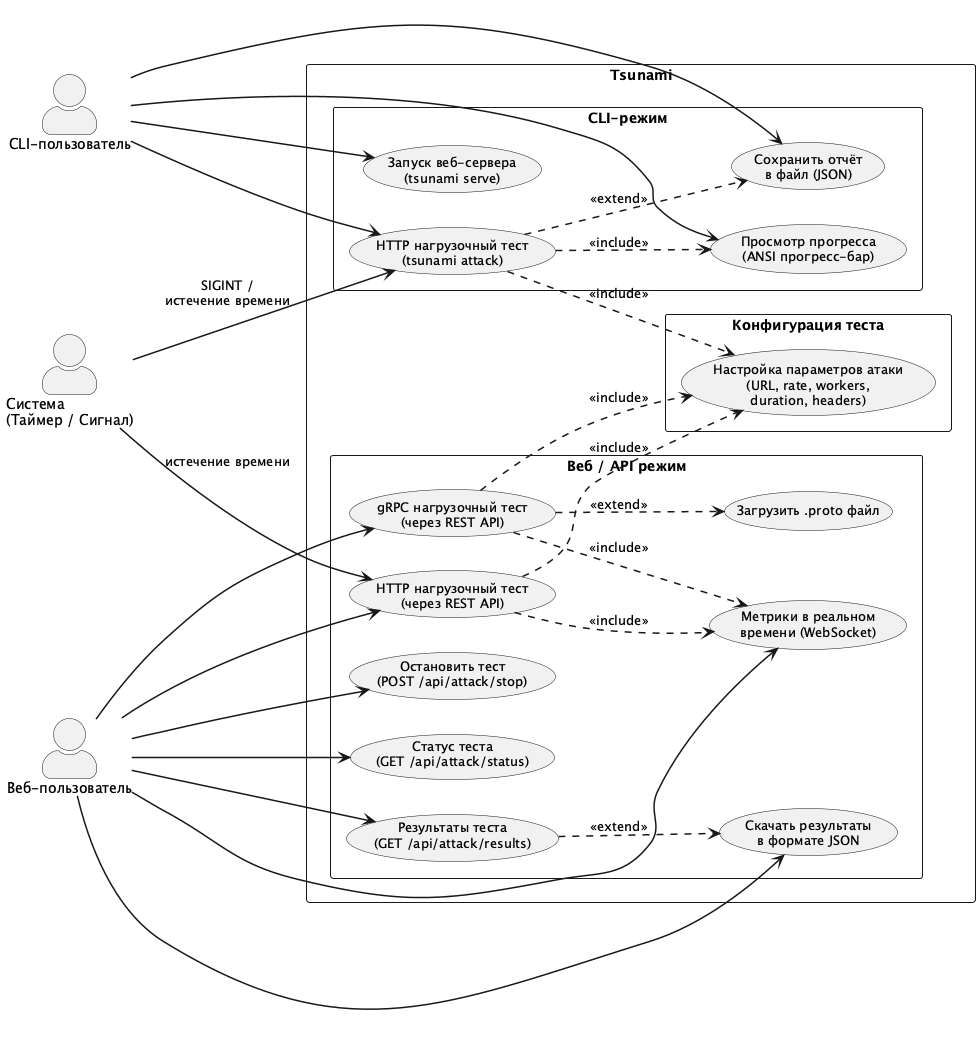
\includegraphics[width=0.92\linewidth]{assets/images/fig-01-tsunami-usecase.png}
  \caption{Диаграмма прецедентов системы Tsunami}
  \label{fig:ch1-usecase}
\end{figure}

CLI-пользователь взаимодействует с системой через команды \texttt{attack},
\texttt{serve} и \texttt{grpc}, получает живой прогресс в терминале
и сохраняет отчёт в файл.
Веб-пользователь управляет тестами через браузерный интерфейс,
получает метрики в реальном времени по протоколу WebSocket,
останавливает тест вручную и скачивает результаты.
Обе категории пользователей используют общий модуль конфигурации атаки.


\section{Выбор технологий и архитектурных решений}

Обоснованный выбор технологического стека является необходимым условием достижения
поставленных функциональных и нефункциональных требований.
В данном разделе приводится сравнительный анализ альтернатив и обоснование
принятых решений по каждому компоненту системы.

\subsection*{Язык программирования}

Для реализации ядра инструмента рассматривались три языка: Go, Python и Rust.

\textbf{Python} обладает развитой экосистемой для сетевого программирования
(asyncio, aiohttp), однако глобальная блокировка интерпретатора (GIL) ограничивает
параллельное выполнение CPU-нагрузки в нескольких потоках.
Кроме того, Python-приложение требует наличия интерпретатора на целевой машине,
что противоречит нефункциональному требованию о поставке единым бинарным файлом.

\textbf{Rust} обеспечивает наивысшую производительность и гарантии безопасности памяти
на уровне системы типов, однако обладает высоким порогом вхождения
и значительно увеличивает время разработки по сравнению с Go.

\textbf{Go} был выбран как оптимальный язык по совокупности характеристик~\cite{gospec}:
\begin{itemize}
  \item горутины~--- легковесные потоки исполнения с начальным размером стека ~2~КБ,
    позволяющие эффективно реализовать пул из сотен параллельных воркеров;
  \item встроенные примитивы конкурентности~--- каналы (\texttt{chan}),
    пакет \texttt{sync}, контексты (\texttt{context.Context})~---
    обеспечивают безопасную координацию горутин;
  \item статическая компиляция в единый бинарный файл без рантайм-зависимостей
    при установке флага \texttt{CGO\_ENABLED=0};
  \item богатая стандартная библиотека: \texttt{net/http} с пулом соединений,
    \texttt{crypto/tls}, \texttt{encoding/json};
  \item простая кросс-компиляция под любую целевую платформу через переменные окружения
    \texttt{GOOS} и \texttt{GOARCH}.
\end{itemize}

\subsection*{CLI-фреймворк}

Для организации интерфейса командной строки сравнивались библиотеки
\texttt{spf13/cobra} и \texttt{urfave/cli}.

\texttt{urfave/cli} предоставляет простой API, достаточный для однокомандных утилит,
однако слабо поддерживает вложенные субкоманды и не имеет встроенной
генерации документации.

\texttt{cobra}~--- стандарт де-факто для CLI-инструментов в экосистеме Go,
используется в таких проектах, как Docker, Kubernetes, Helm и GitHub CLI~\cite{cobra}.
Библиотека предоставляет гибкую систему субкоманд, автоматическую генерацию
справочного текста, поддержку персистентных флагов и хуки \texttt{PersistentPreRun}
для валидации входных параметров.
По результатам сравнения выбрана библиотека \texttt{cobra}.

\subsection*{Ограничение частоты запросов}

Для точного управления скоростью отправки запросов рассматривались три подхода:
\texttt{time.Ticker} из стандартной библиотеки, \texttt{golang.org/x/time/rate}
(алгоритм token bucket) и \texttt{go.uber.org/ratelimit} (алгоритм leaky bucket).

\texttt{time.Ticker} генерирует тики с фиксированным интервалом, однако при задержке
обработки тики накапливаются, что приводит к пиковым всплескам запросов
вместо равномерного потока.

\texttt{golang.org/x/time/rate} реализует token bucket: токены накапливаются
при простое и могут быть истрачены за один такт в режиме burst, что нежелательно
при воспроизводимом нагрузочном тестировании.

\texttt{go.uber.org/ratelimit} реализует алгоритм leaky bucket~\cite{ratelimit}:
метод \texttt{Take()} блокирует вызывающую горутину до момента, когда следующий
токен может быть выдан, обеспечивая строго равномерное распределение запросов
во времени.
Именно такое поведение критично для нагрузочного тестирования, где требуется
воспроизводимая постоянная нагрузка с заданным RPS.
Выбрана библиотека \texttt{go.uber.org/ratelimit}.

\subsection*{WebSocket}

Для реализации потоковой передачи метрик в реальном времени сравнивались
библиотеки \texttt{gorilla/websocket} и \texttt{nhooyr.io/websocket}.

\texttt{nhooyr.io/websocket}~--- более новая библиотека с контекстно-ориентированным API,
однако с меньшей зрелостью и значительно меньшим сообществом пользователей.

\texttt{gorilla/websocket}~--- наиболее широко применяемая Go-реализация протокола
WebSocket~\cite{gorilla}, используется в тысячах производственных проектов.
Библиотека обеспечивает полное соответствие RFC~6455, поддержку компрессии
и гибкую настройку параметров соединения.
По результатам сравнения выбрана \texttt{gorilla/websocket}.

\subsection*{Поддержка gRPC}

Поддержка gRPC реализована на основе официального Go-пакета
\texttt{google.golang.org/grpc}~\cite{grpcgo}~---
единственного зрелого gRPC-фреймворка для Go, поддерживаемого командой Google.
Для динамической компиляции .proto-файлов без использования внешнего компилятора
\texttt{protoc} применяется библиотека \texttt{bufbuild/protocompile},
предоставляющая программный интерфейс к компилятору Protocol Buffers.
Это позволяет пользователям передавать .proto-файлы непосредственно во время
выполнения теста без предварительной генерации кода.

\subsection*{Фронтенд}

Для разработки веб-интерфейса рассматривались три фреймворка: Angular, Vue.js и React.

\textbf{Angular}~--- полнофункциональный фреймворк с встроенными средствами управления
состоянием и строгой структурой проекта.
Для одностраничного дашборда мониторинга Angular является избыточным:
высокий порог вхождения и большой объём итогового бандла не соответствуют
требованию о встраивании фронтенда непосредственно в Go-бинарь.

\textbf{Vue.js}~--- прогрессивный фреймворк с простым API, однако экосистема библиотек
для визуализации данных в реальном времени уступает React-экосистеме по зрелости
и разнообразию компонентов.

\textbf{React}~18 в связке с TypeScript~5 был выбран как оптимальное решение~\cite{react}:
компонентный подход обеспечивает модульность, богатая экосистема предоставляет
готовые решения для всех задач, а строгая типизация TypeScript снижает
вероятность ошибок в рантайме.
Для визуализации метрик выбрана библиотека \textbf{Recharts}~---
декларативная SVG-библиотека графиков, органично интегрирующаяся с React.
Стилизация реализована с помощью \textbf{Tailwind CSS}, обеспечивающего
утилитарный подход к оформлению без необходимости писать отдельные CSS-файлы.

Встраивание скомпилированного React SPA в Go-бинарь выполнено с помощью
директивы \texttt{//go:embed}, что позволяет распространять единый исполняемый файл,
содержащий как серверную, так и клиентскую часть приложения~\cite{gospec}.

Итоговый технологический стек представлен в таблице~\ref{tab:ch1-stack}.

\begin{table}[tbp]
  \centering
  \caption{Технологический стек инструмента Tsunami}
  \label{tab:ch1-stack}
  \begin{tabular}{@{}p{0.22\linewidth}p{0.28\linewidth}p{0.42\linewidth}@{}}
    \toprule
    Компонент        & Технология                   & Обоснование выбора \\
    \midrule
    Язык бэкенда     & Go 1.25                      & Горутины, статический бинарь, кросс-компиляция \\
    CLI-фреймворк    & Cobra v1.10                  & Стандарт де-факто; субкоманды, хуки, генерация справки \\
    Rate limiting    & uber/ratelimit v0.3           & Leaky bucket; строго равномерный поток запросов \\
    WebSocket        & gorilla/websocket v1.5       & RFC~6455, зрелая библиотека, production-ready \\
    gRPC             & google.golang.org/grpc v1.80 & Официальный Go gRPC-фреймворк от Google \\
    Компилятор proto & bufbuild/protocompile v0.14  & Динамическая компиляция .proto без protoc \\
    UI-фреймворк     & React 18 + TypeScript 5      & Компонентность, экосистема, типобезопасность \\
    Графики          & Recharts 2.10                & Декларативные SVG-графики, интеграция с React \\
    CSS-фреймворк    & Tailwind CSS 3.4             & Утилитарный подход, малый итоговый бандл \\
    Встраивание SPA  & go:embed                     & Единый бинарь без внешних статических файлов \\
    Сборщик          & Vite 5                       & Быстрая сборка, нативная поддержка TypeScript \\
    \bottomrule
  \end{tabular}
\end{table}


\section{Проектирование архитектуры системы}

На основе сформулированных требований и выбранного технологического стека была
спроектирована трёхслойная архитектура инструмента Tsunami.

\subsection*{Компонентная структура}

Система состоит из трёх основных слоёв.

\textbf{CLI-слой} (\texttt{cmd/}) реализован на основе фреймворка Cobra и включает
три субкоманды: \texttt{attack} (HTTP-тестирование), \texttt{grpc}
(gRPC-тестирование) и \texttt{serve} (запуск веб-сервера).
Слой отвечает за парсинг флагов командной строки, валидацию входных параметров
и вывод результатов в терминал или файл.

\textbf{Движок нагрузочного тестирования} (\texttt{internal/attack/},
\texttt{internal/grpcattack/}) является ядром системы.
Содержит конфигурационные структуры (\texttt{AttackConfig}), пул воркеров,
диспетчер задач с ограничением скорости, потокобезопасный сборщик метрик
(\texttt{GlobalMetrics}) и генератор JSON-отчётов.

\textbf{HTTP-сервер с веб-интерфейсом} (\texttt{cmd/server/}) предоставляет
REST~API для управления тестами, WebSocket-хаб для стриминга метрик
и встроенное React-приложение.

Принципиально важным архитектурным решением является то, что CLI-слой
и HTTP-сервер используют один и тот же движок нагрузочного тестирования.
Это исключает дублирование бизнес-логики и гарантирует идентичное поведение
системы вне зависимости от способа управления~--- через терминал или браузер.

\subsection*{Паттерн «пул воркеров»}

Движок нагрузочного тестирования построен на паттерне «пул воркеров»
с каналами задач и результатов (рисунок~\ref{fig:ch1-workerpool}).

\begin{figure}[tbp]
  \centering
  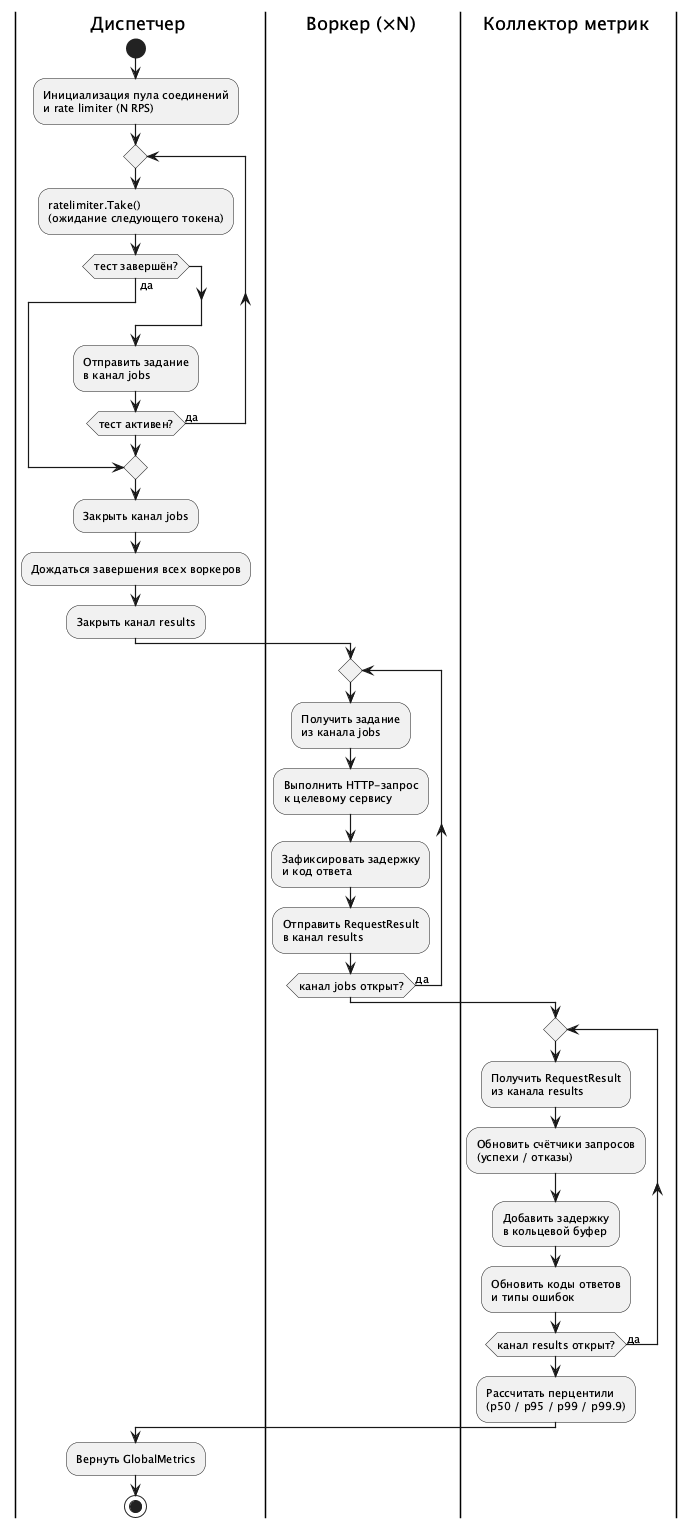
\includegraphics[width=\linewidth,height=0.72\textheight,keepaspectratio]{assets/images/fig-02-tsunami-workerpool.png}
  \caption{Схема взаимодействия компонентов движка нагрузочного тестирования}
  \label{fig:ch1-workerpool}
\end{figure}

Диспетчер задач в цикле вызывает метод \texttt{ratelimiter.Take()},
который блокирует выполнение до наступления следующего разрешённого момента
согласно алгоритму leaky bucket.
После получения токена диспетчер помещает задание в буферизованный канал \texttt{jobs}.

$N$ горутин-воркеров одновременно ожидают заданий из канала \texttt{jobs}.
Получив задание, каждый воркер выполняет HTTP- или gRPC-запрос к целевому сервису,
фиксирует время ответа и помещает объект \texttt{RequestResult} в канал \texttt{results}.
Структура \texttt{RequestResult} содержит код ответа, задержку, признак успеха,
тип ошибки и объём переданных данных.

Горутина-коллектор последовательно считывает результаты из канала \texttt{results}
и накапливает их в структуре \texttt{GlobalMetrics}, защищённой мьютексом.
Такое разделение ответственности позволяет воркерам не блокироваться на операциях
агрегации метрик и достигать высокой пропускной способности.

\subsection*{Структура GlobalMetrics и расчёт перцентилей}

Структура \texttt{GlobalMetrics} обеспечивает потокобезопасный сбор всех метрик теста.
Для хранения значений задержки используется кольцевой буфер
(\texttt{Latencies []time.Duration}) ёмкостью 100\,000~элементов.
При каждом добавлении нового значения индекс сдвигается по модулю размера буфера,
что гарантирует ограниченное потребление оперативной памяти
вне зависимости от длительности теста и числа запросов.

Перцентили задержки (p50, p95, p99, p99.9) вычисляются по завершении теста
функцией \texttt{CalculateAllPercentiles}: буфер сортируется однократно,
после чего значения перцентилей считываются из соответствующих позиций
отсортированного массива.
Однократная сортировка вместо четырёх независимых вызовов снижает вычислительную
сложность с $O(4 \cdot n \log n)$ до $O(n \log n)$.

Для построения временного графика задержки используется отдельный буфер
\texttt{LatencyHistory} ёмкостью 1\,000~точек: сэмплирование выполняется
каждые~10 запросов, что обеспечивает равномерное покрытие всего интервала теста
вне зависимости от его продолжительности.

\subsection*{Конечный автомат TestSession}

При управлении тестом через веб-интерфейс жизненный цикл каждого испытания
контролируется объектом \texttt{TestSession}, реализующим конечный автомат
с пятью состояниями (рисунок~\ref{fig:ch1-statemachine}).

\begin{figure}[tbp]
  \centering
  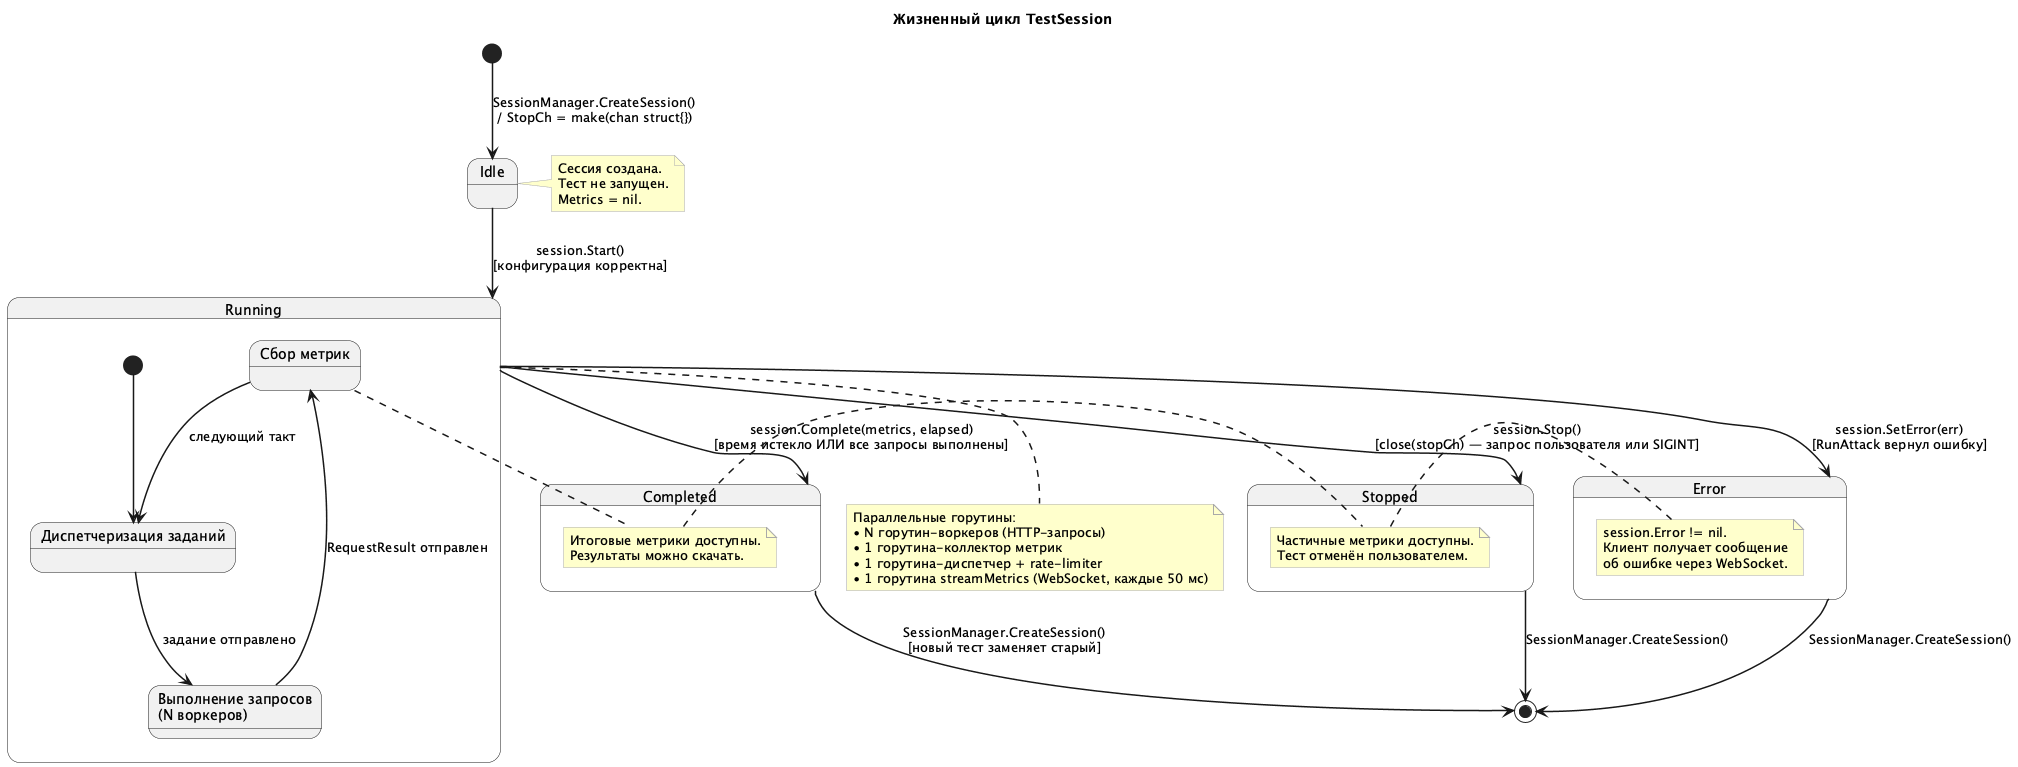
\includegraphics[width=0.80\linewidth]{assets/images/fig-03-tsunami-statemachine.png}
  \caption{Диаграмма состояний объекта TestSession}
  \label{fig:ch1-statemachine}
\end{figure}

В состоянии \textbf{Idle} сессия создана, но тест ещё не запущен.
Переход в состояние \textbf{Running} происходит при вызове метода
\texttt{session.Start()}.
Из состояния Running возможны три перехода:
в \textbf{Completed}~--- по истечении заданной длительности теста;
в \textbf{Stopped}~--- при явной остановке пользователем через REST~API;
в \textbf{Error}~--- при возникновении критической ошибки в движке атаки.

Остановка теста реализована через канал \texttt{StopCh} типа \texttt{chan struct{}}.
Закрытие канала является неблокирующим широковещательным сигналом для всех горутин,
которые отслеживают его состояние через конструкцию \texttt{select}.

\subsection*{WebSocket-хаб и стриминг метрик}

Для трансляции метрик подключённым браузерным клиентам применяется
паттерн «хаб» (\texttt{Hub}).
Хаб поддерживает три канала: \texttt{register}, \texttt{unregister} и \texttt{broadcast}.
Горутина \texttt{Hub.Run()} в цикле обрабатывает эти каналы:
регистрирует новых клиентов, удаляет отключившихся и рассылает сообщения
всем активным соединениям.

Отдельная горутина \texttt{streamMetrics} с интервалом 50~мс считывает текущее
состояние \texttt{GlobalMetrics}, формирует объект \texttt{MetricsPayload}
и передаёт его в канал \texttt{broadcast} хаба.
Каждый клиент имеет собственный буферизованный канал \texttt{send} ёмкостью
256~сообщений и отдельные горутины \texttt{readPump}/\texttt{writePump},
что предотвращает блокировку хаба при наличии медленных или зависших клиентов.

\subsection*{REST API сервера}

HTTP-сервер предоставляет следующие эндпоинты (таблица~\ref{tab:ch1-api}):

\begin{table}[tbp]
  \centering
  \caption{Эндпоинты REST API инструмента Tsunami}
  \label{tab:ch1-api}
  \begin{tabular}{@{}p{0.10\linewidth}p{0.34\linewidth}p{0.48\linewidth}@{}}
    \toprule
    Метод & Путь & Описание \\
    \midrule
    POST & \texttt{/api/attack/start}            & Запуск нагрузочного теста \\
    POST & \texttt{/api/attack/stop}             & Остановка текущего теста \\
    GET  & \texttt{/api/attack/status}           & Текущий статус и метрики теста \\
    GET  & \texttt{/api/attack/results}          & Итоговые результаты после завершения \\
    GET  & \texttt{/api/attack/results/download} & Скачать результаты в формате JSON \\
    POST & \texttt{/api/proto/upload}            & Загрузить .proto-файл для gRPC \\
    WS   & \texttt{/ws/metrics}                  & WebSocket: стриминг метрик (50~мс) \\
    GET  & \texttt{/health}                      & Проверка работоспособности сервера \\
    \bottomrule
  \end{tabular}
\end{table}

Маршрутизация организована таким образом, что все запросы к путям \texttt{/api/},
\texttt{/ws/} и \texttt{/health} обрабатываются API-мультиплексором,
а все остальные пути передаются обработчику SPA (\texttt{SPAHandler}),
который возвращает \texttt{index.html} для поддержки клиентской маршрутизации React.
К серверу применяется CORS-middleware, разрешающий кросс-доменные запросы
в режиме разработки.

Таким образом, спроектированная архитектура обеспечивает чёткое разделение
ответственности между слоями: CLI и веб-сервер используют единый движок
нагрузочного тестирования, что исключает дублирование бизнес-логики.
Применение паттернов пула воркеров, конечного автомата и WebSocket-хаба
позволяет достичь высокой производительности и удобства мониторинга в реальном времени.
Принятые в данной главе архитектурные решения реализуются в главе~2.


\chapter{Проектная часть}
Вторая глава показывает расширенные конструкции. Для удобства чтения сохраняется тот же
принцип: от математического блока к табличному, затем к коду и алгоритмам. Такой порядок
помогает новичку видеть, как сложные окружения собираются в единую структуру текста ВКР.

\section{Многострочная математика и ограничения}
\subsection{Целевая функция и ограничения}
Для продвинутого примера рассматривается задача минимизации целевой функции
с набором ограничений:
\begin{align}
  \min_{x_1,x_2,x_3}\; Z &= 4x_1 + 3x_2 + 2x_3,
  \label{eq:ch2-objective} \\
  x_1 + x_2 + x_3 &= 1, \label{eq:ch2-constraint-a} \\
  2x_1 + x_2 &\ge 0.80, \label{eq:ch2-constraint-b} \\
  x_i &\ge 0,\quad i=1,2,3. \label{eq:ch2-constraint-c}
\end{align}
Формулы~\eqref{eq:ch2-objective}--\eqref{eq:ch2-constraint-c} используются как единый
связанный блок, где каждая строка имеет отдельную ссылку.

\subsection{Рекуррентная модель и режимы}
Дополнительная рекуррентная модель записывается как
\begin{gather}
  F_0 = 1,\quad F_1 = 1, \label{eq:ch2-rec-a} \\
  F_n = F_{n-1} + F_{n-2},\quad n \ge 2. \label{eq:ch2-rec-b}
\end{gather}

Режим вычисления выбирается по условию:
\begin{equation}
  \operatorname{Mode}(u)=
  \begin{cases}
    \text{offline}, & u < 0.40, \\
    \text{hybrid}, & 0.40 \le u < 0.75, \\
    \text{online}, & u \ge 0.75.
  \end{cases}
  \label{eq:ch2-mode}
\end{equation}

\section{Демонстрация длинной таблицы}
\subsection{Реестр контрольных прогонов}
Длинная таблица~\ref{tab:ch2-long} иллюстрирует работу `longtable` при переносе
на несколько страниц и аккуратное выравнивание чисел:
\begin{longtable}{@{}clS[table-format=2.2]S[table-format=1.2]@{}}
  \caption{Реестр контрольных прогонов по этапам проекта}\label{tab:ch2-long} \\
  \toprule
  № & Этап & {Длительность, ч} & {Индекс качества} \\
  \midrule
  \endfirsthead
  \caption[]{Реестр контрольных прогонов по этапам проекта (продолжение)} \\
  \toprule
  № & Этап & {Длительность, ч} & {Индекс качества} \\
  \midrule
  \endhead
  \midrule
  \multicolumn{4}{r}{Продолжение на следующей странице} \\
  \endfoot
  \bottomrule
  \endlastfoot
  1  & Сбор требований                     & 12.50 & 0.78 \\
  2  & Проектирование структуры            & 10.00 & 0.81 \\
  3  & Подготовка титульного листа         & 5.50  & 0.88 \\
  4  & Настройка шрифтов                   & 6.25  & 0.92 \\
  5  & Разметка формул                     & 8.75  & 0.85 \\
  6  & Разметка рисунков                   & 7.00  & 0.86 \\
  7  & Разметка таблиц                     & 9.25  & 0.87 \\
  8  & Реализация листингов                & 6.50  & 0.90 \\
  9  & Реализация алгоритмов               & 7.40  & 0.91 \\
  10 & Настройка перекрестных ссылок       & 4.80  & 0.95 \\
  11 & Тестирование пайплайна              & 6.10  & 0.96 \\
  12 & Корректировка методических пояснений& 5.70  & 0.89 \\
  13 & Подготовка приложений               & 7.90  & 0.90 \\
  14 & Финальный прогон сборки             & 3.60  & 0.98 \\
  15 & Предзащитная валидация              & 4.20  & 0.97 \\
\end{longtable}

\subsection{Архитектурная иллюстрация}
Дополнительная архитектурная иллюстрация приведена на рисунке~\ref{fig:ch2-cache};
она показывает роль кэш-уровня в снижении латентности запроса.
Источник диаграммы: открытый репозиторий системного проектирования~\cite{sdp-cache}.
\begin{figure}[tbp]
  \centering
  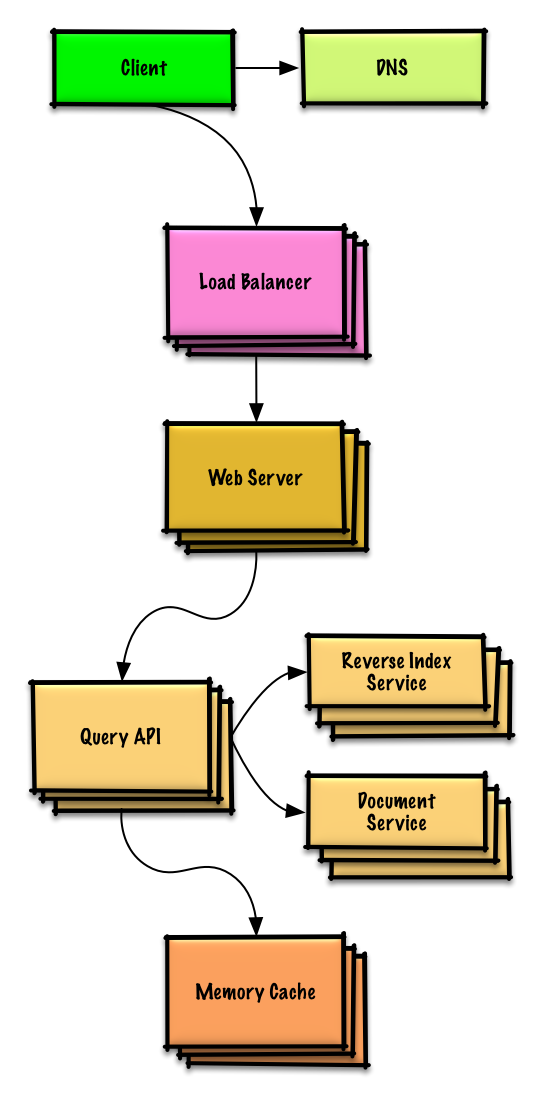
\includegraphics[width=0.64\linewidth]{assets/images/fig-04-query-cache-architecture.png}
  \caption{Архитектура кэширования запросов в распределенном сервисе}
  \label{fig:ch2-cache}
\end{figure}

\section{Демонстрация листингов}
\subsection{Python-листинг проверки структуры}
Листинг~\ref{lst:ch2-validator} показывает рабочий пример кода, который
обходит каталог контента и проверяет наличие ожидаемых файлов:
\begin{lstlisting}[caption={Скрипт валидации структуры контента},label={lst:ch2-validator}]
from pathlib import Path

CONTENT_FILES = [
    "01-introduction.tex",
    "02-chapter-1.tex",
    "03-chapter-2.tex",
    "04-conclusion.tex",
]

root = Path("content")
missing = [name for name in CONTENT_FILES if not (root / name).exists()]

if missing:
    print("Missing files:", ", ".join(missing))
else:
    print("Content structure is valid.")
\end{lstlisting}

\subsection{Bash-фрагмент сборочного сценария}
Для демонстрации конфигурационного фрагмента используется листинг~\ref{lst:ch2-make-target}:
\begin{lstlisting}[language=bash,caption={Пример цели Makefile для сборки},label={lst:ch2-make-target}]
build:
	latexmk -pdf -lualatex main.tex
\end{lstlisting}

\subsection{LaTeX-листинги шаблонов}
Листинги LaTeX оформляются с локальным указанием языка, чтобы новичкам было проще
сопоставлять окружения, команды и метки:
\begin{lstlisting}[language={[LaTeX]TeX},texcsstyle=*\color{lstKeyword},alsoletter={\\},morekeywords={begin,end,chapter,section,subsection,label,ref,eqref,caption,includegraphics},caption={Шаблон нумеруемой формулы с меткой},label={lst:ch2-latex-equation}]
\begin{equation}
  S = \sum_{i=1}^{n} w_i x_i,
  \label{eq:weighted-score}
\end{equation}
\end{lstlisting}

\begin{lstlisting}[language={[LaTeX]TeX},texcsstyle=*\color{lstKeyword},alsoletter={\\},morekeywords={begin,end,chapter,section,subsection,label,ref,eqref,caption,includegraphics},caption={Шаблон рисунка с подписью и ссылкой},label={lst:ch2-latex-figure}]
\begin{figure}[tbp]
  \centering
  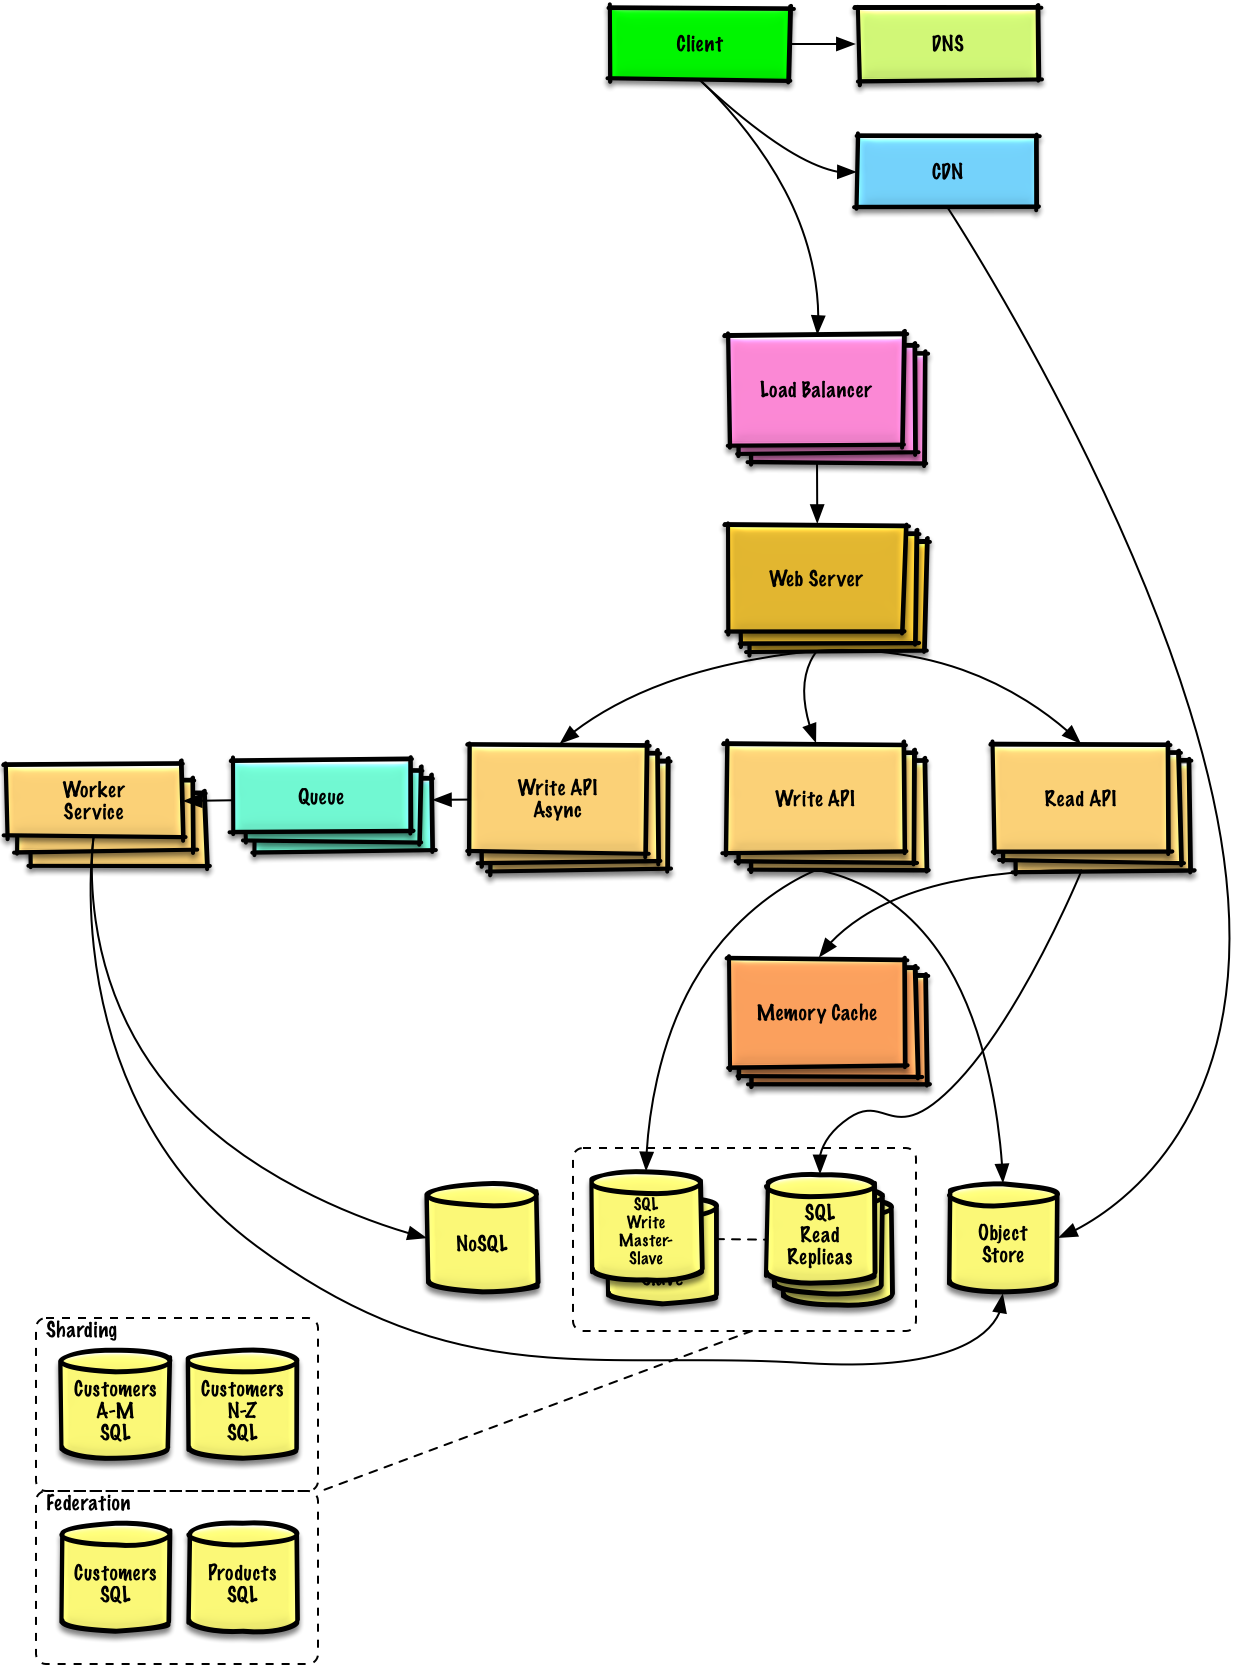
\includegraphics[width=0.8\linewidth]{assets/images/fig-05-aws-scaling-architecture.png}
  \caption{Схема масштабирования сервиса в облачной среде}
  \label{fig:scaling-demo}
\end{figure}
\end{lstlisting}

\section{Демонстрация алгоритмов}
\subsection{Псевдокод формирования отчета}
Алгоритм~\ref{alg:ch2-report} демонстрирует псевдокод построения отчета качества:
\begin{algorithm}[tbp]
  \caption{Формирование отчета контроля сборки}
  \label{alg:ch2-report}
  \begin{algorithmic}[1]
    \Require Массив `checks`, содержащий статусы проверок
    \Ensure Текстовый отчет `report`
    \State `passed` $\gets$ 0
    \State `report` $\gets$ пустой список
    \ForAll{элемент `check` в `checks`}
      \If{`check.status` = ``ok''}
        \State `passed` $\gets$ `passed` + 1
        \State добавить строку ``OK: check.name'' в `report`
      \Else
        \State добавить строку ``FAIL: check.name'' в `report`
      \EndIf
    \EndFor
    \State добавить итог ``passed / |checks|'' в `report`
    \State \Return `report`
  \end{algorithmic}
\end{algorithm}

\section{Композитный кейс 2: полный advanced-блок}
\subsection{Интеграция сложных элементов}
Для демонстрации сквозного сценария в одной связке используются:
формула оптимизации~\eqref{eq:ch2-objective}, длинная таблица~\ref{tab:ch2-long},
листинг валидации~\ref{lst:ch2-validator}, алгоритм~\ref{alg:ch2-report}
и визуальные схемы~\ref{fig:ch1-subfig},~\ref{fig:ch2-cache}.

\subsection{Практические ориентиры по оформлению}
Кейс показывает, что даже при усложнении синтаксиса документ остается управляемым:
каждый элемент имеет устойчивую ссылку, подпись и воспроизводимую сборку.
Для практики рекомендуется опираться на официальные справочники пакетов
`listings`, `algorithmicx` и `siunitx`~\cite{listings-doc,algpseudocode-doc,siunitx-doc},
а также на общую методологию literate programming~\cite{knuth1984}
и примеры архитектурных схем открытого сообщества~\cite{sdp-repo,sdp-aws}.


\makeconclusion
В ходе выпускной квалификационной работы была достигнута поставленная цель:
разработаны CLI-инструмент и веб-интерфейс для системы нагрузочного тестирования
HTTP и gRPC сервисов, обеспечивающие гибкое управление нагрузкой
и визуализацию метрик в реальном времени.

В процессе выполнения работы были решены следующие задачи.

Проведён сравнительный анализ существующих инструментов нагрузочного
тестирования~--- Apache JMeter, Gatling, k6, Vegeta и hey.
В ходе анализа установлено, что ни один из рассмотренных инструментов
не сочетает в себе распространение в виде единого бинарного файла, поддержку HTTP и gRPC
в одном дистрибутиве и встроенный веб-интерфейс с потоковой передачей метрик,
что обусловило необходимость разработки инструмента Tsunami.

Сформулированы функциональные и нефункциональные
требования к разрабатываемому инструменту.
Среди ключевых нефункциональных требований: поставка единым бинарным файлом,
кросс-платформенная поддержка шести платформ, целевая производительность
не менее 1000~RPS при 50 параллельных исполнителях и задержка WebSocket-трансляции
не более 100~мс.

Спроектирована трёхслойная архитектура системы, включающая движок нагрузочного
тестирования, CLI-слой на базе Cobra и HTTP-сервер с WebSocket-сервером.
Для формализации проектных решений разработаны диаграммы прецедентов, классов,
состояний и последовательности.

Реализован движок нагрузочного тестирования с поддержкой HTTP и gRPC.
Движок построен по паттерну «резерв исполнителей» с ограничителем скорости
на алгоритме текущего ведра.
Потокобезопасный сбор метрик обеспечивается кольцевым буфером ёмкостью
100\,000~замеров; по завершении теста вычисляются перцентили задержки
P50, P90, P95 и P99 за одну сортировки.
Реализована классификация сетевых ошибок по пяти категориям,
что позволяет оперативно отличить инфраструктурные сбои от прикладных ошибок сервера.

Реализованы CLI-интерфейс и веб-интерфейс системы для управления нагрузочными
тестами и мониторинга метрик в реальном времени.
CLI-интерфейс на базе Cobra включает команды \texttt{attack}, \texttt{serve}
и \texttt{grpc} с настраиваемой интенсивностью запросов и штатным завершением теста.
Веб-интерфейс реализован как React SPA с графиками Recharts и встраивается
в исполняемый файл через директиву \texttt{//go:embed};
REST~API из восьми маршрутов и WebSocket-сервер с интервалом трансляции 50~мс
обеспечивают управление тестами и потоковую передачу метрик через браузер.

Проведено двухуровневое тестирование системы.
Юнит-тесты функции \texttt{CalculateAllPercentiles} охватывают 13~сценариев,
включая граничные случаи.
Интеграционные тесты с библиотекой testcontainers-go используют реальный
Docker-контейнер с сервисом httpbin и верифицируют точность классификации ошибок,
корректность счётчиков метрик и соответствие REST~API заявленным контрактам.
Все тесты успешно проходят в среде GitHub Actions~CI.

\textbf{Практическая ценность} разработанного инструмента Tsunami состоит в том,
что он обеспечивает нагрузочное тестирование HTTP и gRPC сервисов в виде
единого самодостаточного бинарного файла без зависимостей среды выполнения,
распространяемого для шести целевых платформ через GitHub Releases и Homebrew.
Инструмент готов к применению инженерами по качеству и DevOps-специалистами
в профессиональной деятельности, в том числе в составе автоматизированных
конвейеров CI/CD.

Перспективными направлениями развития инструмента являются поддержка сценарного
нагрузочного тестирования с переменной интенсивностью, интеграция трассировки
через OpenTelemetry и реализация распределённого режима нагрузки
с несколькими агентами.


\printgostbibliography

\makeappendicesblock
\appendixchapterfirst{А}{Шаблоны математических окружений}
В приложении собраны минимальные шаблоны математических конструкций, использованных
в главах 1 и 2. Блок можно копировать в собственный текст с заменой обозначений.

\begin{lstlisting}[language={[LaTeX]TeX},texcsstyle=*\color{lstKeyword},alsoletter={\\},morekeywords={begin,end,chapter,section,subsection,label,ref,eqref,caption,includegraphics},caption={Базовые шаблоны формул},label={lst:app-a-formulas}]
\begin{equation}
  y = kx + b,
  \label{eq:sample-linear}
\end{equation}

\begin{align}
  x_{norm} &= \frac{x - x_{\min}}{x_{\max} - x_{\min}}, \label{eq:sample-a} \\
  score &= 0.6 x_{norm} + 0.4 q. \label{eq:sample-b}
\end{align}

\begin{equation}
  f(x)=
  \begin{cases}
    0, & x < 0, \\
    1, & x \ge 0.
  \end{cases}
  \label{eq:sample-case}
\end{equation}
\end{lstlisting}

\appendixchapternext{Б}{Шаблоны рисунков и таблиц}
В приложении представлен полный текст конфигурационного файла GoReleaser
\texttt{.goreleaser.yaml}, управляющего кросс-компиляцией, упаковкой артефактов,
публикацией релизов на GitHub и обновлением Homebrew-формулы.

\begin{lstlisting}[language={},caption={Конфигурация GoReleaser (\texttt{.goreleaser.yaml})},label={lst:app-goreleaser}]
version: 2

project_name: tsunami

before:
  hooks:
    - go mod tidy

builds:
  - id: tsunami
    main: ./main.go
    binary: tsunami
    env:
      - CGO_ENABLED=0
    goos:
      - linux
      - darwin
      - windows
    goarch:
      - amd64
      - arm64
    ldflags:
      - -s -w
      - -X github.com/paniccaaa/tsunami/cmd.Version={{.Version}}
    tags:
      - netgo
      - embed_frontend

archives:
  - id: default
    builds:
      - tsunami
    name_template: >-
      {{ .ProjectName }}_{{ .Version }}_{{ .Os }}_{{ .Arch }}
    format_overrides:
      - goos: windows
        format: zip

checksum:
  name_template: "checksums.txt"
  algorithm: sha256

changelog:
  sort: asc
  filters:
    exclude:
      - "^docs:"
      - "^test:"
      - "^chore:"
      - "Merge pull request"
      - "Merge branch"

brews:
  - name: tsunami
    repository:
      owner: paniccaaa
      name: homebrew-tap
      token: "{{ .Env.HOMEBREW_TAP_TOKEN }}"
    directory: Formula
    homepage: "https://github.com/paniccaaa/tsunami"
    description: "HTTP load testing CLI tool"
    license: "MIT"
    install: |
      bin.install "tsunami"
    test: |
      system "#{bin}/tsunami", "--version"

release:
  github:
    owner: paniccaaa
    name: tsunami
  draft: false
  prerelease: auto
  name_template: "v{{.Version}}"
\end{lstlisting}

\appendixchapternext{В}{Шаблоны листингов и алгоритмов}
В приложении представлен полный исходный код интеграционных тестов движка
нагрузочного тестирования из файла \texttt{tests/integration/attack\_test.go}.
Тесты используют библиотеку testcontainers-go для запуска реального
Docker-контейнера с сервисом httpbin и верифицируют корректность
метрик, классификации ошибок и обработки HTTP-статусов.

\begin{lstlisting}[language=Go,caption={Интеграционные тесты движка (\texttt{tests/integration/attack\_test.go})},label={lst:app-integration}]
//go:build integration

package integration_test

import (
    "testing"
    "time"

    "github.com/paniccaaa/tsunami/internal/attack"
)

func TestRunAttack_BasicSuccess(t *testing.T) {
    cfg := &attack.AttackConfig{
        URL:         testBaseURL + "/get",
        Method:      "GET",
        RPS:         10,
        Duration:    2 * time.Second,
        Workers:     5,
        Connections: 10,
        Timeout:     5 * time.Second,
    }
    stopCh := make(chan struct{})
    metrics, elapsed, err := attack.RunAttack(cfg, stopCh)
    if err != nil {
        t.Fatalf("RunAttack failed: %v", err)
    }
    if metrics.TotalRequests == 0 {
        t.Error("expected TotalRequests > 0")
    }
    if metrics.Failures > 0 {
        t.Errorf("expected 0 failures, got %d", metrics.Failures)
    }
    if metrics.StatusCodes[200] == 0 {
        t.Error("expected 200 status codes to be counted")
    }
    if metrics.TotalRequests != metrics.Successes {
        t.Errorf("all requests should be successful: total=%d successes=%d",
            metrics.TotalRequests, metrics.Successes)
    }
    if elapsed == 0 {
        t.Error("expected elapsed time > 0")
    }
    if metrics.MaxLatency == 0 {
        t.Error("expected MaxLatency to be recorded")
    }
    if metrics.MinLatency >= metrics.MaxLatency && metrics.TotalRequests > 1 {
        t.Errorf("expected MinLatency < MaxLatency, got min=%v max=%v",
            metrics.MinLatency, metrics.MaxLatency)
    }
}

func TestRunAttack_TimeoutClassification(t *testing.T) {
    cfg := &attack.AttackConfig{
        URL:         testBaseURL + "/delay/3",
        Method:      "GET",
        RPS:         5,
        Duration:    2 * time.Second,
        Workers:     5,
        Connections: 10,
        Timeout:     500 * time.Millisecond,
    }
    stopCh := make(chan struct{})
    metrics, _, err := attack.RunAttack(cfg, stopCh)
    if err != nil {
        t.Fatalf("RunAttack failed: %v", err)
    }
    if metrics.Failures == 0 {
        t.Error("expected failures due to timeout, got 0")
    }
    if metrics.Successes > 0 {
        t.Errorf("expected 0 successes, got %d", metrics.Successes)
    }
    if metrics.ErrorTypes[attack.ErrorTypeTimeout] == 0 {
        t.Errorf("expected ErrorTypeTimeout, got: %v", metrics.ErrorTypes)
    }
    for errType, count := range metrics.ErrorTypes {
        if errType != attack.ErrorTypeTimeout && count > 0 {
            t.Errorf("unexpected error type %q: %d", errType, count)
        }
    }
}

func TestRunAttack_MetricsAccuracy(t *testing.T) {
    t.Run("2xx is a success", func(t *testing.T) {
        cfg := &attack.AttackConfig{
            URL: testBaseURL + "/status/201", Method: "GET",
            RPS: 10, Duration: 2 * time.Second,
            Workers: 5, Connections: 10,
            Timeout: 5 * time.Second,
        }
        stopCh := make(chan struct{})
        metrics, _, err := attack.RunAttack(cfg, stopCh)
        if err != nil { t.Fatalf("RunAttack failed: %v", err) }
        if metrics.Successes == 0 {
            t.Error("expected Successes > 0 for /status/201")
        }
        if metrics.Failures > 0 {
            t.Errorf("expected 0 Failures for /status/201, got %d", metrics.Failures)
        }
        if metrics.StatusCodes[201] == 0 {
            t.Error("expected 201 to be tracked in StatusCodes")
        }
    })
    t.Run("5xx is a failure", func(t *testing.T) {
        cfg := &attack.AttackConfig{
            URL: testBaseURL + "/status/500", Method: "GET",
            RPS: 10, Duration: 2 * time.Second,
            Workers: 5, Connections: 10,
            Timeout: 5 * time.Second,
        }
        stopCh := make(chan struct{})
        metrics, _, err := attack.RunAttack(cfg, stopCh)
        if err != nil { t.Fatalf("RunAttack failed: %v", err) }
        if metrics.Failures == 0 {
            t.Error("expected Failures > 0 for /status/500")
        }
        if metrics.StatusCodes[500] == 0 {
            t.Error("expected 500 to be tracked in StatusCodes")
        }
        if len(metrics.ErrorTypes) > 0 {
            t.Errorf("HTTP 500 should not produce ErrorType entries, got: %v",
                metrics.ErrorTypes)
        }
    })
    t.Run("4xx is a failure", func(t *testing.T) {
        cfg := &attack.AttackConfig{
            URL: testBaseURL + "/status/404", Method: "GET",
            RPS: 10, Duration: 2 * time.Second,
            Workers: 5, Connections: 10,
            Timeout: 5 * time.Second,
        }
        stopCh := make(chan struct{})
        metrics, _, err := attack.RunAttack(cfg, stopCh)
        if err != nil { t.Fatalf("RunAttack failed: %v", err) }
        if metrics.Failures == 0 {
            t.Error("expected Failures > 0 for /status/404")
        }
        if metrics.StatusCodes[404] == 0 {
            t.Error("expected 404 to be tracked in StatusCodes")
        }
    })
}
\end{lstlisting}

\appendixchapternext{Г}{Чеклист перед финальной сборкой}
В приложении представлен пример JSON-отчёта, экспортируемого инструментом Tsunami
по завершении нагрузочного теста.
Отчёт соответствует структуре \texttt{MetricsReport} из пакета \texttt{internal/attack}
и содержит конфигурацию теста, сводную статистику, перцентили задержки,
распределение HTTP-статусов и разбивку ошибок по типам.

\begin{lstlisting}[language={},caption={Пример JSON-отчёта результатов нагрузочного теста},label={lst:app-report}]
{
  "config": {
    "url": "https://example.com/api/v1/status",
    "method": "GET",
    "duration": "30s",
    "timeout": "10s",
    "workers": 50,
    "connections": 100,
    "rps": 500
  },
  "summary": {
    "total_requests": 14987,
    "successful_requests": 14952,
    "failed_requests": 35,
    "total_elapsed_time": "30s",
    "average_latency": "48ms",
    "min_latency": "12ms",
    "max_latency": "1204ms",
    "throughput_rps": 499.57,
    "target_rps": 500,
    "bytes_sent": 0,
    "bytes_received": 10840264
  },
  "latency_percentiles": {
    "p50": "41ms",
    "p90": "87ms",
    "p95": "132ms",
    "p99": "389ms"
  },
  "status_codes": {
    "200": 14952,
    "429": 22,
    "503": 13
  },
  "error_breakdown": {
    "timeout": 35,
    "connection_refused": 0,
    "dns": 0,
    "tls": 0,
    "other": 0
  },
  "timestamp": "2026-04-22T14:35:07+03:00"
}
\end{lstlisting}


\end{document}
